\section{Auswertung}
\label{sec:Auswertung}

\subsection{Impuls-Echo-Verfahren}

In Tabelle \ref{tab:echo} sind für die verschieden langen Zylinder mit dem A-Scan gemessenen Laufzeiten und Amplituden des ersten und zweiten Pulses aufgelistet.
\begin{table}
  \centering
  \caption{Laufzeiten und Amplituden für das Impuls-Echo-Verfahren.}
  \label{tab:echo}
  \begin{tabular}{c | c c | c c | c}
    \toprule
    & \multicolumn{2}{c}{Puls 1} & \multicolumn{2}{c}{Puls 2} & \\
    Länge [\si{\centi\meter}] & $U$ [\si{\volt}] & $t$ [\si{\micro\second}] & $U$ [\si{\volt}] & $t$ [\si{\micro\second}] & $\increment t$ [\si{\micro\second}] \\
    \midrule
    11,9 & 1,486 & 0,4 & 0,922 & 89,2 & 88,8 \\
     7,9 & 1,486 & 0,4 & 1,385 & 60,2 & 59,8 \\
     3,7 & 1,486 & 0,4 & 1,457 & 29,7 & 29,3 \\
      10 & 1,486 & 0,4 & 1,173 & 76,6 & 76,6 \\
     5,9 & 1,486 & 0,4 & 1,415 &   46 & 45,4 \\
       8 (kombiniert) & 1,486 & 0,4 & 1,366 &   60 & 59,6 \\
     3,1 & 1,486 & 0,4 & 1,456 & 23,6 & 23,2 \\
    \bottomrule
  \end{tabular}
\end{table}

\subsubsection{Schallgeschwindigkeit}
\label{sec:geschw}

Die Schallgeschwindigkeit kann nicht direkt mit Gleichung \eqref{eqn:gl4} besimmt werden, da die Laufzeiten aufgrund Anpassungsschicht einen systematischen Fehler besitzen.
Deshalb wird eine lineare Ausgleichsrechnung durchgeführt (siehe Abb. \ref{fig:plot1}).
\begin{equation}
  y(x) = A \cdot x + B
\end{equation}
\begin{figure}
  \includegraphics{build/plot1.pdf}
  \caption{linearer Zusammenhang zwischen Laufzeit und der Länge der Zylinder für das Impuls-Echo-Verfahren.}
  \label{fig:plot1}
\end{figure}
Die Steigung dieser Geraden enspricht der Schallgeschwindigkeit und deren Nullstelle der doppelten Laufzeit durch die Anpassungsschicht.
\begin{align*}
  A_\text{Echo} &= c_\text{Echo} = \SI{2697(40)}{\meter\per\second} \\
  B_\text{Echo} &= \SI{0.42(24)}{\centi\meter} \\
  t_\text{Anpassung,Echo} &= - \frac{B_\text{Echo}}{2 \cdot A_\text{Echo}} =\SI{0.77}{\micro\second}
\end{align*}
Die Schallgeschwindigkeit in der Anpassungsschicht ist nicht bekannt.
Da die Anpassungsschicht jedoch dazu dient, den Übergang des Schalls in das Acryl zu erleichtern, kann für die Anpassungsschicht eine ähnliche Schallgeschwindigkeit angenommen werden.
So kann aus der Laufzeit folgende Dicke bestimmt werden.
\begin{equation*}
d_\text{Echo} = c_\text{Echo} \cdot t_\text{Anpassung,Echo} = \SI{0.21}{\centi\meter}
\end{equation*}

\subsubsection{Dämpfung}

Um die Dämpfung zu berechnen, wird Gleichung \eqref{eqn:gl3} umgestellt werden.
\begin{equation}
 \alpha = -\frac{\ln(I(x)/I_0)}{x}
\end{equation}
Mit den Werten aus Tabelle \ref{tab:echo} werden die Absorptionskoeffizienten berechnet.
\begin{align*}
  \alpha_1 &= \SI{4.01}{\per\meter} \\
  \alpha_2 &= \SI{0.89}{\per\meter} \\
  \alpha_3 &= \SI{0.53}{\per\meter} \\
  \alpha_4 &= \SI{2.37}{\per\meter} \\
  \alpha_5 &= \SI{0.83}{\per\meter} \\
  \alpha_6 &= \SI{1.05}{\per\meter} \\
  \alpha_7 &= \SI{10.66}{\per\meter} \\
  \bar\alpha &= \SI{1.48}{\per\meter}
\end{align*}

\subsection{Durchschallungsverfahren}

Mit dem Durchschallungsverfahren soll ebenfalls die Schallgeschwindigkeit bestimmt werden, folgende Laufzeiten werden dabei gemessen (siehe Tabelle \ref{tab:Durch}).
\begin{table}
  \centering
  \caption{Laufzeiten für das Durchschallungsverfahren.}
  \label{tab:Durch}
  \begin{tabular}{c c}
    \toprule
    Länge [\si{\centi\meter}] & $t$ [\si{\micro\second}] \\
    \midrule
    11,9  & 45,9 \\
     7,9  & 31,5 \\
     3,7  & 15,9 \\
      10  & 40,5 \\
     5,9  & 24,2 \\
       8 (kombiniert) & 31,3 \\
     3,1  & 12,6 \\
    \bottomrule
  \end{tabular}
\end{table}
Analog zum Impuls-Echo-Verfahren wird eine Ausgleichsrechnung mit Gleichung \eqref{eqn:gl4} durchgeführt (siehe Abb. \ref{fig:plot2}).
\begin{figure}
  \includegraphics{build/plot2.pdf}
  \caption{linearer Zusammenhang zwischen Laufzeit und der Länge der Zylinder für das Durchschallungsverfahren.}
  \label{fig:plot2}
\end{figure}
Allerdings fällt der Faktor $1/2$ weg, da der Schall den Zylinder nur einmal durchläuft.
Die Steigung dieser Geraden enspricht der Schallgeschwindigkeit und deren Nullstelle der Laufzeit durch die Anpassungsschicht.
\begin{align*}
  A_\text{Durchschallung} &= c_\text{Durchschallung} = \SI{2627(64)}{\meter\per\second} \\
  B_\text{Durchschallung} &= \SI{0.36(20)}{\centi\meter} \\
  t_\text{Anpassung,Durchschallung} &= - \frac{B_\text{Durchschallung}}{2 \cdot A_\text{Durchschallung}} =\SI{0.69}{\micro\second}
\end{align*}
Aus der Laufzeit kann folgende Dicke bestimmt werden.
\begin{equation*}
d_\text{Durchschallung} = c_\text{Durchschallung} \cdot t_\text{Anpassung,Durchschallung} = \SI{0.18}{\centi\meter}
\end{equation*}

\subsection{Spekrale Analyse und Cepstrum}
\label{sec:cep}

Aus Abbildung \ref{fig:cep} lassen sich drei Reflexionen erkennen, aus deren Laufzeiten sich mit Gleichung \eqref{eqn:gl4} die Dicke der Acrylscheiben bestimmen lässt.
Zur Berechnung wird die Schallgeschwindigkeit aus \ref{sec:geschw} benutzt.
\begin{table}
  \centering
  \caption{Laufzeiten der Reflexionen und berechnete Dicke der Scheiben.}
  \label{tab:cep}
  \begin{tabular}{c c c}
    \toprule
    & $t$ [\si{\micro\second}] & Dicke der Scheiben $d$ [\si{\centi\meter}] \\
    \midrule
    Scheibe oben & 4,23 & 0,57\\
    Scheibe unten & 7,16 & 0,97\\
    Scheiben zusammen & 11,41 & 1,54 \\
    \bottomrule
  \end{tabular}
\end{table}
\begin{figure}
  \centering
  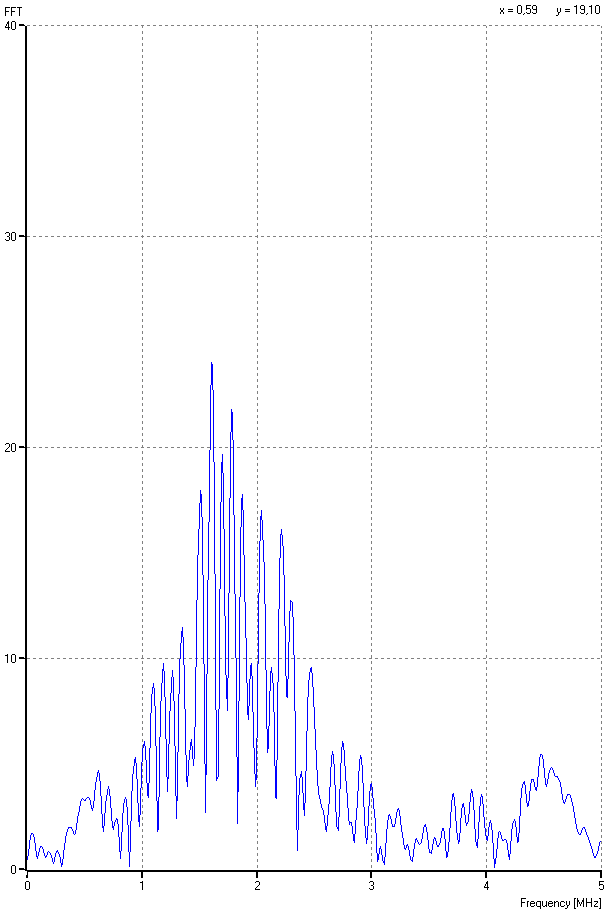
\includegraphics[height=8cm]{data/FFT.png}
  \caption{Spektrum der Ultraschallsonde.}
  \label{fig:FFT}
\end{figure}
\begin{figure}
  \centering
  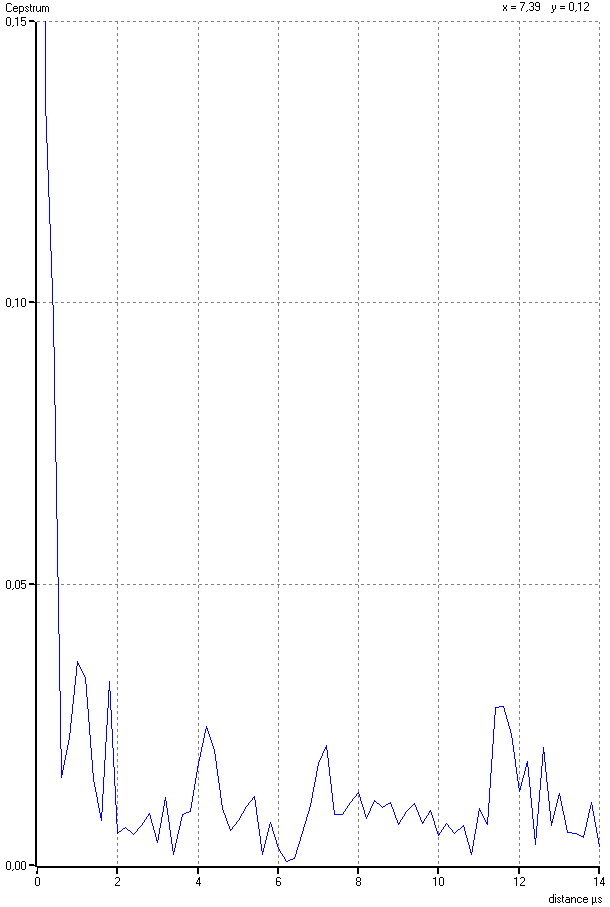
\includegraphics[height=8cm]{data/Cepstrum.png}
  \caption{Cepstrum der Ultraschallsonde.}
  \label{fig:cep}
\end{figure}

\FloatBarrier

\subsection{Abmessungen des Auges}

Im richtigen Einschallwinkel lassen sich 4 Reflexionen im Auge messen (siehe Tabelle \ref{tab:Auge}), die an den Grenzflächen der verschiedenen Augenbestandteile auftreten.
\begin{table}
  \centering
  \caption{Laufzeiten der Echos im Auge.}
  \label{tab:Auge}
  \begin{tabular}{c c c c}
    \toprule
    $t_1$ (Iris) & $t_2$ (Linse Eingang) & $t_3$ (Linse Ausgang) & $t_4$ (Retina) \\
    \midrule
    \SI{11.7}{\micro\second} & \SI{16.2}{\micro\second} & \SI{23.6}{\micro\second} & \SI{73}{\micro\second} \\
    \bottomrule
  \end{tabular}
\end{table}
Die Schallgeschwindigkeit der Glaskörperflüssigkeit beträgt $c_\text{GK} = \SI{1410}{\meter\per\second}$ und in der Linse $c_\text{L} = \SI{2500}{\meter\per\second}$.
Bevor die Abstände mit Gleichung \eqref{eqn:gl4} berechnet werden können, muss die Laufzeit bis zur Iris zweimal um die Laufzeit der Anpassungsschicht korrigiert werden.
\begin{table}
  \centering
  \caption{Laufzeiten der Echos im Auge.}
  \label{tab:Auge}
  \begin{tabular}{c c c c c}
    \toprule
    von & zu & Laufzeit $\increment t$ & Abmessung Augenmodell & Abmessung echtes Auge (1:3) \\
    \midrule
    Hornhaut & Iris & \SI{10.16}{\micro\second} & \SI{7.16}{\milli\meter} & \SI{2.39}{\milli\meter}  \\
    Iris & Linse Eingang & \SI{4.5}{\micro\second} & \SI{3.17}{\milli\meter} & \SI{1.06}{\milli\meter} \\
    Linse Eingang & Linse Ausgang & \SI{7.4}{\micro\second} & \SI{9.25}{\milli\meter} & \SI{3.08}{\milli\meter} \\
    Linse Ausgang & Retina & \SI{49.4}{\micro\second} & \SI{3.48}{\centi\meter} & \SI{1.16}{\centi\meter} \\
    Hornhaut & Retina & & \SI{5.44}{\centi\meter} & \SI{1.81}{\centi\meter} \\
    \bottomrule
  \end{tabular}
\end{table}
